\documentclass[conference]{IEEEtran}
\usepackage{graphicx}
\usepackage[cmex10]{amsmath}
\usepackage{enumitem}
\usepackage{tikz}
\usepackage[backend=biber,style=ieee,bibstyle=authortitle,sorting=none]{biblatex}
\addbibresource{lib.bib}

\begin{document}

\title{Automatically generating data associations over different file types}
\author{\IEEEauthorblockN{Marcus Schlutter}
\IEEEauthorblockA{Siemens AG\\
		  Chemnitz, Germany\\
		  marcus.schlutter@etit.tu-chemnitz.de}
}

\maketitle

\begin{abstract}
This document proposes an algorithm to match file content / data associations in different file
types for the purpose to use the associations to generate one file from the other. The proposal
is independent from the underlying data but dependents on the arrangment of the data which
must support a path-like addressing scheme to select the correct path based on simple majority.
The principle is shown on a scenario where data is present in multiple docx-files and a single
XML-file with the objective to generate the XML-file.
\end{abstract}

\begin{IEEEkeywords}
Machine Learning-like, file generation, data associations, Office-digitalization, XML
\end{IEEEkeywords}

\section{Introduction}
The presence of programs like \textit{Datatap} \cite{adverity:adverity} or \textit{MapForce}
\cite{altova:mapforce} show that there's a demand for programs which are capable of of extracting
data from one file (format) to another. Both solutions however lack the automization in the
meaning of the manual interaction is required to create associations. Here an approach is proposed
to overcome this limitation by automatically create associations without the application of
neuronal networks in favor of traceability.\\
The proposal is first explained in an abstract manner in the \textit{Procedure}-section and
will later shown on an example which should given the reader a much better grasp of the
implementation.

\section{Requirements}
For the proposed algorithm to work as expected some prerequisite have to be formulated:
\begin{enumerate}[label=(\roman*)]
% \item The data to be associated represents complex data structures which occur multiple
%        times ie. it is a list of objects
 \item Files should be separable into 2 groups: one being the \textit{target}-group containing
        only one file \footnote{technically multiple files should be possible but this is
        discouraged}. While the other group is the \textit{source}-group
 \item Both groups contain the same data represented in complex structures which occur multiple
        times ie. it is a list of objects. For the \textit{source}-group this can be only a
        subset of the data available.
 \item In both groups the contained data is arranged in a way that every field of this complex
        data structures can be addressed individually.
 \item The data within this data structures need to be heterogenous (between the different
        fields)
\end{enumerate}

\section{Procedure}
The algorithm can be separated in 3 functional steps: the collection-phase, the selection-phase
and the generation (of the \textit{target}-file).\\All steps build one a central internal data
structure which can be visualized as a 2-dimensional histogram which stores path-pairs as their
occurances.

\subsection{Collection-Phase}
All values available in the first file ie. \textit{target}-file are to be extracted and
paired with their addressing path. Paths should be constructed independent of the current
complex structure but specific to they field they represent.
\begin{figure}[h]
  \centering
 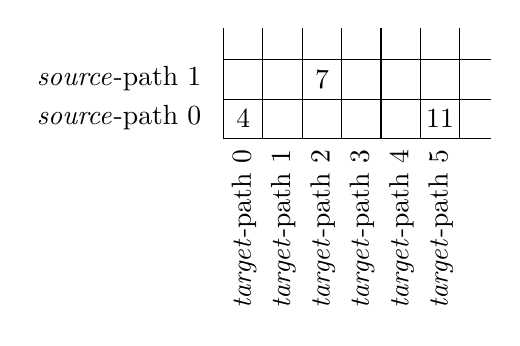
\begin{tikzpicture}
  \draw (1,2.4) -- (1,1) -- (4.4,1);
  \draw[step=0.5] (1,1) grid (4.4,2.4);
  \foreach \x/\i in {1.1/0, 1.6/1, 2.1/2, 2.6/3, 3.1/4, 3.6/5}
    \node[label={[label distance=-6.5em, text depth=-1ex,rotate=90]right: \textit{target}-path \i}]
            at (\x,1) {};
  \foreach \y/\i in {1.3/0, 1.8/1}
    \node[label={[label distance=1, text depth=-1ex]left: \textit{source}-path \i}]
            at (1,\y) {};
  \node at (1.25,1.25) {4};
  \node at (2.25,1.75) {7};
  \node at (3.75,1.25) {11};
 \end{tikzpicture}
 \caption{2-dimensional histogram for storing path-pairs}
 \label{classifier_table}
\end{figure}
In the next step this collection is compared against the values in the group of
\textit{source}-file(s) were every match is recorded in the forementioned 2-dimensional histogram.
Figure \ref{classifier_table} shows an examplary arrangment. In the next step the collected data
is evaluated.

\subsection{Selection-Phase}
In this step from all the possible path combinations the correct one shall be selected. This is
resolved considering the problem as a simple case of the \textit{Byzantine Generals Problem} as
described in \cite{lamport:byzantine}. From this also the limitations of the algorithm can be derived:
for every path-match $p_i$ $p$ is derived as $majority(p_1, p_2, ...,p_n)$ under the assumption that
$n \geq 2k + 1$ with $k$ being the count of errors. An error manifests either as a wrong path-pair due
to the value is matched multiple times for different data structure fields or a correct match could
not be made due to the \textit{target}-file containing a false value (compared to the content of the
corresponding \textit{source}-file).

\subsection{Generation}
After all matches had been made correctly (intervention is possible by manually altering the
histogram-structure) the \textit{target}-file can be derived from the \textit{source}-files in
case the later are modified or extended. Structural changes can be compensated by ``re-training''
the system.\\As the main goal of the algorithm is to pick the right ``bin'' in the histogram it
has been named \textit{Naive BinClassifier}.

\section{Implementation example}
To outline the core principles and give a better understanding of applying the proposed algorithm
to real world problems this chapter presents the implementation steps for transforming tables in
form of docx-files into a XML-file. Both contain data of a ficticious company.\\The XML-file will
contain only a subset of the information provided by multiple docx-files. For ease of
implementation the nodes of interest were provided via a configuration file: the company sections
and the list of workers.\\
In the docx-files data was distributed over multiple sheets with one column that referenced to
another file. The assignment of workers to their sections is arranged in a so called cross-table:
the workers listed on the side, the sections listed on the top and the spanned rectangle is filled
with 'x' at the correct place. All table-headers are separated by the actual data by a different
background of cell.

\subsection{Project organisation}
\begin{figure}[h]
 \centering
 \includegraphics[scale=0.3]{img/ProjectStructure_en}
 \caption{Project organisation for example project}
 \label{project_structure}
\end{figure}

Both file types need to be addressable via path: this was achieved by creating specialized
wrapper-classes as shown in figure \ref{project_structure}. For XML XPath could be applied, for
docx a path was constructed using the filename, the sheet name and cell addressing with column and
row. To detect the type of table in the docx-file the different types are tried and the correct
selection is left to the classifier.
\begin{figure}[ht]
 \centering
 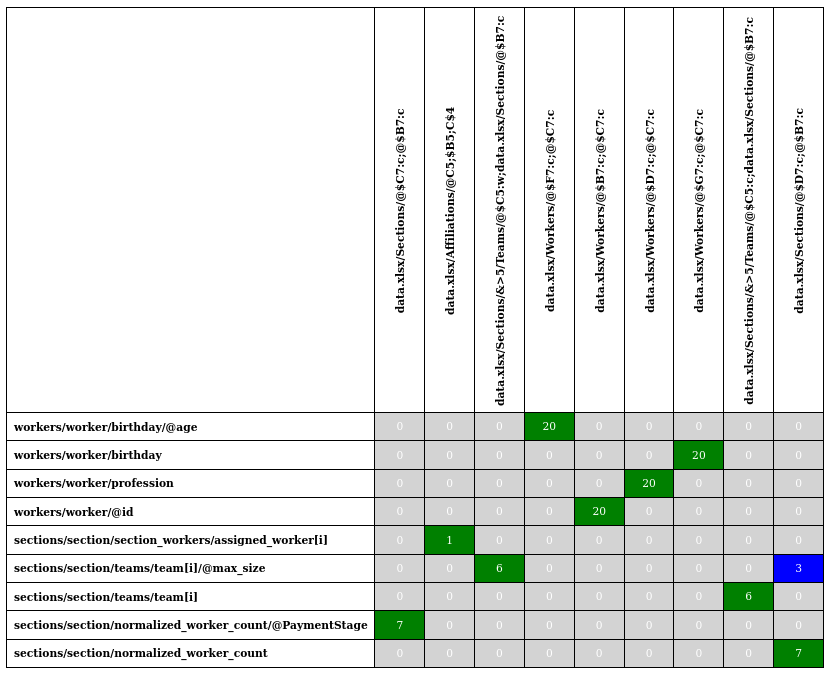
\includegraphics[scale=0.39]{img/example_table}
 \caption{Collection and Selection result for 20 workers distributed over 6 sections}
 \label{example_table}
\end{figure}
As figure \ref{example_table} shows does this yield good results. For generating the XML file in
the later process the original XML was stripped of the matched paths (which was namely the worker
and section parts) and assumed constant. For the given scenario a worker count below 11 broke the
algorithm as values became to homogenous.

\section{Summary}
In this document an algorithm was presented which is capable of ``learning'' data associations
between different file types called \textit{Naive BinClassifier}. This algorithm decides over
associations by majority of path-pairings which worked well in a case study presented as an
example.

\printbibliography

\end{document}
